\documentclass[1p]{elsarticle_modified}
%\bibliographystyle{elsarticle-num}

%\usepackage[colorlinks]{hyperref}
%\usepackage{abbrmath_seonhwa} %\Abb, \Ascr, \Acal ,\Abf, \Afrak
\usepackage{amsfonts}
\usepackage{amssymb}
\usepackage{amsmath}
\usepackage{amsthm}
\usepackage{scalefnt}
\usepackage{amsbsy}
\usepackage{kotex}
\usepackage{caption}
\usepackage{subfig}
\usepackage{color}
\usepackage{graphicx}
\usepackage{xcolor} %% white, black, red, green, blue, cyan, magenta, yellow
\usepackage{float}
\usepackage{setspace}
\usepackage{hyperref}

\usepackage{tikz}
\usetikzlibrary{arrows}

\usepackage{multirow}
\usepackage{array} % fixed length table
\usepackage{hhline}

%%%%%%%%%%%%%%%%%%%%%
\makeatletter
\renewcommand*\env@matrix[1][\arraystretch]{%
	\edef\arraystretch{#1}%
	\hskip -\arraycolsep
	\let\@ifnextchar\new@ifnextchar
	\array{*\c@MaxMatrixCols c}}
\makeatother %https://tex.stackexchange.com/questions/14071/how-can-i-increase-the-line-spacing-in-a-matrix
%%%%%%%%%%%%%%%

\usepackage[normalem]{ulem}

\newcommand{\msout}[1]{\ifmmode\text{\sout{\ensuremath{#1}}}\else\sout{#1}\fi}
%SOURCE: \msout is \stkout macro in https://tex.stackexchange.com/questions/20609/strikeout-in-math-mode

\newcommand{\cancel}[1]{
	\ifmmode
	{\color{red}\msout{#1}}
	\else
	{\color{red}\sout{#1}}
	\fi
}

\newcommand{\add}[1]{
	{\color{blue}\uwave{#1}}
}

\newcommand{\replace}[2]{
	\ifmmode
	{\color{red}\msout{#1}}{\color{blue}\uwave{#2}}
	\else
	{\color{red}\sout{#1}}{\color{blue}\uwave{#2}}
	\fi
}

\newcommand{\Sol}{\mathcal{S}} %segment
\newcommand{\D}{D} %diagram
\newcommand{\A}{\mathcal{A}} %arc


%%%%%%%%%%%%%%%%%%%%%%%%%%%%%5 test

\def\sl{\operatorname{\textup{SL}}(2,\Cbb)}
\def\psl{\operatorname{\textup{PSL}}(2,\Cbb)}
\def\quan{\mkern 1mu \triangleright \mkern 1mu}

\theoremstyle{definition}
\newtheorem{thm}{Theorem}[section]
\newtheorem{prop}[thm]{Proposition}
\newtheorem{lem}[thm]{Lemma}
\newtheorem{ques}[thm]{Question}
\newtheorem{cor}[thm]{Corollary}
\newtheorem{defn}[thm]{Definition}
\newtheorem{exam}[thm]{Example}
\newtheorem{rmk}[thm]{Remark}
\newtheorem{alg}[thm]{Algorithm}

\newcommand{\I}{\sqrt{-1}}
\begin{document}

%\begin{frontmatter}
%
%\title{Boundary parabolic representations of knots up to 8 crossings}
%
%%% Group authors per affiliation:
%\author{Yunhi Cho} 
%\address{Department of Mathematics, University of Seoul, Seoul, Korea}
%\ead{yhcho@uos.ac.kr}
%
%
%\author{Seonhwa Kim} %\fnref{s_kim}}
%\address{Center for Geometry and Physics, Institute for Basic Science, Pohang, 37673, Korea}
%\ead{ryeona17@ibs.re.kr}
%
%\author{Hyuk Kim}
%\address{Department of Mathematical Sciences, Seoul National University, Seoul 08826, Korea}
%\ead{hyukkim@snu.ac.kr}
%
%\author{Seokbeom Yoon}
%\address{Department of Mathematical Sciences, Seoul National University, Seoul, 08826,  Korea}
%\ead{sbyoon15@snu.ac.kr}
%
%\begin{abstract}
%We find all boundary parabolic representation of knots up to 8 crossings.
%
%\end{abstract}
%\begin{keyword}
%    \MSC[2010] 57M25 
%\end{keyword}
%
%\end{frontmatter}

%\linenumbers
%\tableofcontents
%
\newcommand\colored[1]{\textcolor{white}{\rule[-0.35ex]{0.8em}{1.4ex}}\kern-0.8em\color{red} #1}%
%\newcommand\colored[1]{\textcolor{white}{ #1}\kern-2.17ex	\textcolor{white}{ #1}\kern-1.81ex	\textcolor{white}{ #1}\kern-2.15ex\color{red}#1	}

{\Large $\underline{12a_{0871}~(K12a_{0871})}$}

\setlength{\tabcolsep}{10pt}
\renewcommand{\arraystretch}{1.6}
\vspace{1cm}\begin{tabular}{m{100pt}>{\centering\arraybackslash}m{274pt}}
\multirow{5}{120pt}{
	\centering
	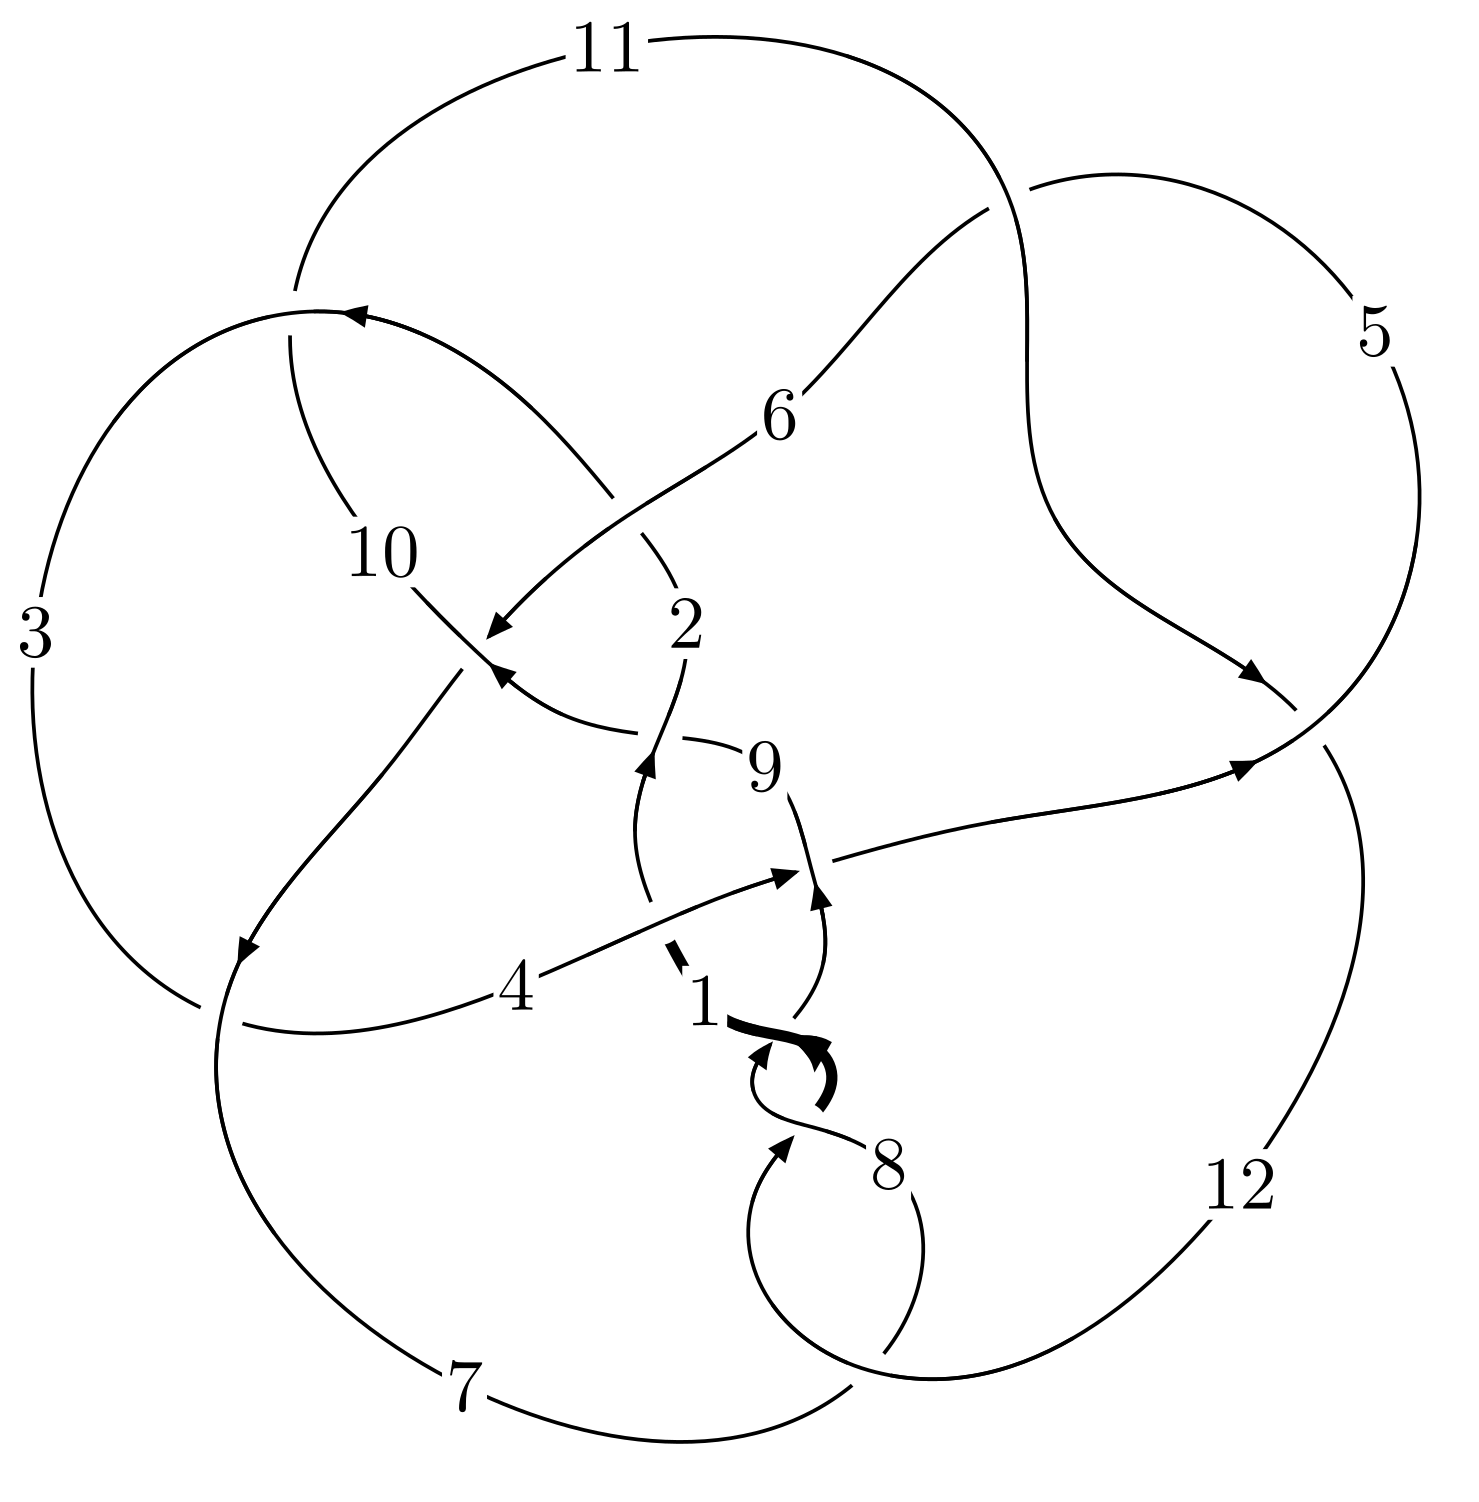
\includegraphics[width=112pt]{../../../GIT/diagram.site/Diagrams/png/1672_12a_0871.png}\\
\ \ \ A knot diagram\footnotemark}&
\allowdisplaybreaks
\textbf{Linearized knot diagam} \\
\cline{2-2}
 &
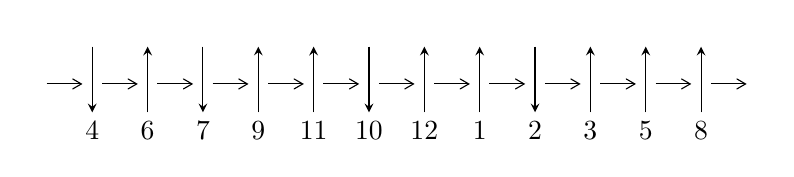
\begin{tikzpicture}[x=20pt, y=17pt]
	% nodes
	\node (C0) at (0, 0) {};
	\node (C1) at (1, 0) {};
	\node (C1U) at (1, +1) {};
	\node (C1D) at (1, -1) {4};

	\node (C2) at (2, 0) {};
	\node (C2U) at (2, +1) {};
	\node (C2D) at (2, -1) {6};

	\node (C3) at (3, 0) {};
	\node (C3U) at (3, +1) {};
	\node (C3D) at (3, -1) {7};

	\node (C4) at (4, 0) {};
	\node (C4U) at (4, +1) {};
	\node (C4D) at (4, -1) {9};

	\node (C5) at (5, 0) {};
	\node (C5U) at (5, +1) {};
	\node (C5D) at (5, -1) {11};

	\node (C6) at (6, 0) {};
	\node (C6U) at (6, +1) {};
	\node (C6D) at (6, -1) {10};

	\node (C7) at (7, 0) {};
	\node (C7U) at (7, +1) {};
	\node (C7D) at (7, -1) {12};

	\node (C8) at (8, 0) {};
	\node (C8U) at (8, +1) {};
	\node (C8D) at (8, -1) {1};

	\node (C9) at (9, 0) {};
	\node (C9U) at (9, +1) {};
	\node (C9D) at (9, -1) {2};

	\node (C10) at (10, 0) {};
	\node (C10U) at (10, +1) {};
	\node (C10D) at (10, -1) {3};

	\node (C11) at (11, 0) {};
	\node (C11U) at (11, +1) {};
	\node (C11D) at (11, -1) {5};

	\node (C12) at (12, 0) {};
	\node (C12U) at (12, +1) {};
	\node (C12D) at (12, -1) {8};
	\node (C13) at (13, 0) {};

	% arrows
	\draw[->,>={angle 60}]
	(C0) edge (C1) (C1) edge (C2) (C2) edge (C3) (C3) edge (C4) (C4) edge (C5) (C5) edge (C6) (C6) edge (C7) (C7) edge (C8) (C8) edge (C9) (C9) edge (C10) (C10) edge (C11) (C11) edge (C12) (C12) edge (C13) ;	\draw[->,>=stealth]
	(C1U) edge (C1D) (C2D) edge (C2U) (C3U) edge (C3D) (C4D) edge (C4U) (C5D) edge (C5U) (C6U) edge (C6D) (C7D) edge (C7U) (C8D) edge (C8U) (C9U) edge (C9D) (C10D) edge (C10U) (C11D) edge (C11U) (C12D) edge (C12U) ;
	\end{tikzpicture} \\
\hhline{~~} \\& 
\textbf{Solving Sequence} \\ \cline{2-2} 
 &
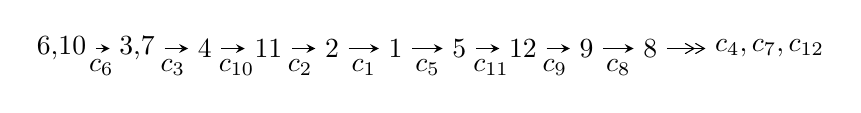
\begin{tikzpicture}[x=23pt, y=7pt]
	% node
	\node (A0) at (-1/8, 0) {6,10};
	\node (A1) at (17/16, 0) {3,7};
	\node (A2) at (17/8, 0) {4};
	\node (A3) at (25/8, 0) {11};
	\node (A4) at (33/8, 0) {2};
	\node (A5) at (41/8, 0) {1};
	\node (A6) at (49/8, 0) {5};
	\node (A7) at (57/8, 0) {12};
	\node (A8) at (65/8, 0) {9};
	\node (A9) at (73/8, 0) {8};
	\node (C1) at (1/2, -1) {$c_{6}$};
	\node (C2) at (13/8, -1) {$c_{3}$};
	\node (C3) at (21/8, -1) {$c_{10}$};
	\node (C4) at (29/8, -1) {$c_{2}$};
	\node (C5) at (37/8, -1) {$c_{1}$};
	\node (C6) at (45/8, -1) {$c_{5}$};
	\node (C7) at (53/8, -1) {$c_{11}$};
	\node (C8) at (61/8, -1) {$c_{9}$};
	\node (C9) at (69/8, -1) {$c_{8}$};
	\node (A10) at (11, 0) {$c_{4},c_{7},c_{12}$};

	% edge
	\draw[->,>=stealth]	
	(A0) edge (A1) (A1) edge (A2) (A2) edge (A3) (A3) edge (A4) (A4) edge (A5) (A5) edge (A6) (A6) edge (A7) (A7) edge (A8) (A8) edge (A9) ;
	\draw[->>,>={angle 60}]	
	(A9) edge (A10);
\end{tikzpicture} \\ 

\end{tabular} \\

\footnotetext{
The image of knot diagram is generated by the software ``\textbf{Draw programme}" developed by Andrew Bartholomew(\url{http://www.layer8.co.uk/maths/draw/index.htm\#Running-draw}), where we modified some parts for our purpose(\url{https://github.com/CATsTAILs/LinksPainter}).
}\phantom \\ \newline 
\centering \textbf{Ideals for irreducible components\footnotemark of $X_{\text{par}}$} 
 
\begin{align*}
I^u_{1}&=\langle 
1.80079\times10^{1000} u^{138}+3.01263\times10^{1000} u^{137}+\cdots+9.21046\times10^{999} b+1.47252\times10^{1000},\\
\phantom{I^u_{1}}&\phantom{= \langle  }-3.52539\times10^{999} u^{138}-7.82925\times10^{998} u^{137}+\cdots+9.21046\times10^{999} a-2.10793\times10^{1000},\\
\phantom{I^u_{1}}&\phantom{= \langle  }5 u^{139}+6 u^{138}+\cdots+7 u-1\rangle \\
I^u_{2}&=\langle 
-3.15864\times10^{37} u^{27}-2.23009\times10^{38} u^{26}+\cdots+1.72151\times10^{35} b-1.40370\times10^{37},\\
\phantom{I^u_{2}}&\phantom{= \langle  }-1.15651\times10^{38} u^{27}-8.15998\times10^{38} u^{26}+\cdots+1.72151\times10^{35} a-5.00345\times10^{37},\\
\phantom{I^u_{2}}&\phantom{= \langle  }5 u^{28}+33 u^{27}+\cdots+3 u-1\rangle \\
\\
\end{align*}
\raggedright * 2 irreducible components of $\dim_{\mathbb{C}}=0$, with total 167 representations.\\
\footnotetext{All coefficients of polynomials are rational numbers. But the coefficients are sometimes approximated in decimal forms when there is not enough margin.}
\newpage
\renewcommand{\arraystretch}{1}
\centering \section*{I. $I^u_{1}= \langle 1.80\times10^{1000} u^{138}+3.01\times10^{1000} u^{137}+\cdots+9.21\times10^{999} b+1.47\times10^{1000},\;-3.53\times10^{999} u^{138}-7.83\times10^{998} u^{137}+\cdots+9.21\times10^{999} a-2.11\times10^{1000},\;5 u^{139}+6 u^{138}+\cdots+7 u-1 \rangle$}
\flushleft \textbf{(i) Arc colorings}\\
\begin{tabular}{m{7pt} m{180pt} m{7pt} m{180pt} }
\flushright $a_{6}=$&$\begin{pmatrix}1\\0\end{pmatrix}$ \\
\flushright $a_{10}=$&$\begin{pmatrix}0\\u\end{pmatrix}$ \\
\flushright $a_{3}=$&$\begin{pmatrix}0.382760 u^{138}+0.0850039 u^{137}+\cdots-50.6825 u+2.28863\\-1.95515 u^{138}-3.27088 u^{137}+\cdots+5.78117 u-1.59875\end{pmatrix}$ \\
\flushright $a_{7}=$&$\begin{pmatrix}1\\u^2\end{pmatrix}$ \\
\flushright $a_{4}=$&$\begin{pmatrix}2.22730 u^{138}+3.34356 u^{137}+\cdots-55.8631 u+3.81252\\-1.30760 u^{138}-2.14564 u^{137}+\cdots+4.68692 u-1.38973\end{pmatrix}$ \\
\flushright $a_{11}=$&$\begin{pmatrix}4.67273 u^{138}+7.93391 u^{137}+\cdots-23.1138 u-4.60306\\1.35292 u^{138}+2.48173 u^{137}+\cdots+0.210969 u-0.0658331\end{pmatrix}$ \\
\flushright $a_{2}=$&$\begin{pmatrix}2.33791 u^{138}+3.35588 u^{137}+\cdots-56.4637 u+3.88738\\-1.95515 u^{138}-3.27088 u^{137}+\cdots+5.78117 u-1.59875\end{pmatrix}$ \\
\flushright $a_{1}=$&$\begin{pmatrix}-4.38463 u^{138}-8.32463 u^{137}+\cdots-32.1407 u+2.35356\\-1.10194 u^{138}-2.10304 u^{137}+\cdots+4.27185 u-1.04163\end{pmatrix}$ \\
\flushright $a_{5}=$&$\begin{pmatrix}0.269116 u^{138}+0.793757 u^{137}+\cdots-10.8788 u+4.40556\\-0.861170 u^{138}-1.19922 u^{137}+\cdots-1.11359 u-1.62966\end{pmatrix}$ \\
\flushright $a_{12}=$&$\begin{pmatrix}-14.5571 u^{138}-24.2886 u^{137}+\cdots+59.8087 u-4.14929\\-1.68970 u^{138}-3.29711 u^{137}+\cdots+4.79931 u-0.320587\end{pmatrix}$ \\
\flushright $a_{9}=$&$\begin{pmatrix}3.20950 u^{138}+5.01416 u^{137}+\cdots-23.9423 u-3.84170\\0.110306 u^{138}+0.438015 u^{137}+\cdots+2.61756 u-0.695526\end{pmatrix}$ \\
\flushright $a_{8}=$&$\begin{pmatrix}0.875161 u^{138}+4.27144 u^{137}+\cdots-9.78423 u-1.97659\\1.90839 u^{138}+3.38088 u^{137}+\cdots+3.96701 u-0.143899\end{pmatrix}$\\&\end{tabular}
\flushleft \textbf{(ii) Obstruction class $= -1$}\\~\\
\flushleft \textbf{(iii) Cusp Shapes $= -16.2600 u^{138}-26.4039 u^{137}+\cdots+39.3754 u-2.10248$}\\~\\
\newpage\renewcommand{\arraystretch}{1}
\flushleft \textbf{(iv) u-Polynomials at the component}\newline \\
\begin{tabular}{m{50pt}|m{274pt}}
Crossings & \hspace{64pt}u-Polynomials at each crossing \\
\hline $$\begin{aligned}c_{1}\end{aligned}$$&$\begin{aligned}
&5(5 u^{139}+44 u^{138}+\cdots-138 u+207)
\end{aligned}$\\
\hline $$\begin{aligned}c_{2}\end{aligned}$$&$\begin{aligned}
&u^{139}+23 u^{137}+\cdots+1342610 u+79075
\end{aligned}$\\
\hline $$\begin{aligned}c_{3}\end{aligned}$$&$\begin{aligned}
&u^{139}-4 u^{138}+\cdots+9955539065 u-2811030979
\end{aligned}$\\
\hline $$\begin{aligned}c_{4}\end{aligned}$$&$\begin{aligned}
&u^{139}+u^{138}+\cdots+132792 u-9535
\end{aligned}$\\
\hline $$\begin{aligned}c_{5},c_{11}\end{aligned}$$&$\begin{aligned}
&5(5 u^{139}-6 u^{138}+\cdots+1.08748\times10^{7} u+3500629)
\end{aligned}$\\
\hline $$\begin{aligned}c_{6}\end{aligned}$$&$\begin{aligned}
&5(5 u^{139}-6 u^{138}+\cdots+7 u+1)
\end{aligned}$\\
\hline $$\begin{aligned}c_{7},c_{8},c_{12}\end{aligned}$$&$\begin{aligned}
&u^{139}+u^{138}+\cdots+3436 u+335
\end{aligned}$\\
\hline $$\begin{aligned}c_{9}\end{aligned}$$&$\begin{aligned}
&u^{139}-36 u^{137}+\cdots+911022429 u-918419671
\end{aligned}$\\
\hline $$\begin{aligned}c_{10}\end{aligned}$$&$\begin{aligned}
&u^{139}+2 u^{138}+\cdots-161606 u+44905
\end{aligned}$\\
\hline
\end{tabular}\\~\\
\newpage\renewcommand{\arraystretch}{1}
\flushleft \textbf{(v) Riley Polynomials at the component}\newline \\
\begin{tabular}{m{50pt}|m{274pt}}
Crossings & \hspace{64pt}Riley Polynomials at each crossing \\
\hline $$\begin{aligned}c_{1}\end{aligned}$$&$\begin{aligned}
&25(25 y^{139}-376 y^{138}+\cdots+5015196 y-42849)
\end{aligned}$\\
\hline $$\begin{aligned}c_{2}\end{aligned}$$&$\begin{aligned}
&y^{139}+46 y^{138}+\cdots-50108241400 y-6252855625
\end{aligned}$\\
\hline $$\begin{aligned}c_{3}\end{aligned}$$&$\begin{aligned}
&y^{139}-52 y^{138}+\cdots+2.84\times10^{20} y-7.90\times10^{18}
\end{aligned}$\\
\hline $$\begin{aligned}c_{4}\end{aligned}$$&$\begin{aligned}
&y^{139}- y^{138}+\cdots+15265736154 y-90916225
\end{aligned}$\\
\hline $$\begin{aligned}c_{5},c_{11}\end{aligned}$$&$\begin{aligned}
&25\\
&\cdot(25 y^{139}+2274 y^{138}+\cdots+494385524795298 y-12254403395641)
\end{aligned}$\\
\hline $$\begin{aligned}c_{6}\end{aligned}$$&$\begin{aligned}
&25(25 y^{139}-1076 y^{138}+\cdots+y-1)
\end{aligned}$\\
\hline $$\begin{aligned}c_{7},c_{8},c_{12}\end{aligned}$$&$\begin{aligned}
&y^{139}-133 y^{138}+\cdots-2468254 y-112225
\end{aligned}$\\
\hline $$\begin{aligned}c_{9}\end{aligned}$$&$\begin{aligned}
&y^{139}-72 y^{138}+\cdots+4.72\times10^{19} y-8.43\times10^{17}
\end{aligned}$\\
\hline $$\begin{aligned}c_{10}\end{aligned}$$&$\begin{aligned}
&y^{139}+26 y^{138}+\cdots-67481776374 y-2016459025
\end{aligned}$\\
\hline
\end{tabular}\\~\\
\newpage\flushleft \textbf{(vi) Complex Volumes and Cusp Shapes}
$$\begin{array}{c|c|c}  
\text{Solutions to }I^u_{1}& \I (\text{vol} + \sqrt{-1}CS) & \text{Cusp shape}\\
 \hline 
\begin{aligned}
u &= \phantom{-}0.454159 + 0.925702 I \\
a &= \phantom{-}0.433657 + 1.045870 I \\
b &= -0.556673 + 0.354972 I\end{aligned}
 & \phantom{-}1.56214 - 3.03714 I & \phantom{-0.000000 } 0 \\ \hline\begin{aligned}
u &= \phantom{-}0.454159 - 0.925702 I \\
a &= \phantom{-}0.433657 - 1.045870 I \\
b &= -0.556673 - 0.354972 I\end{aligned}
 & \phantom{-}1.56214 + 3.03714 I & \phantom{-0.000000 } 0 \\ \hline\begin{aligned}
u &= -0.545285 + 0.799666 I \\
a &= -0.76183 + 1.80296 I \\
b &= \phantom{-}0.889411 + 0.684684 I\end{aligned}
 & \phantom{-}3.70539 + 10.84170 I & \phantom{-0.000000 } 0 \\ \hline\begin{aligned}
u &= -0.545285 - 0.799666 I \\
a &= -0.76183 - 1.80296 I \\
b &= \phantom{-}0.889411 - 0.684684 I\end{aligned}
 & \phantom{-}3.70539 - 10.84170 I & \phantom{-0.000000 } 0 \\ \hline\begin{aligned}
u &= \phantom{-}0.579540 + 0.856958 I \\
a &= -0.81515 - 1.44704 I \\
b &= \phantom{-}0.989461 - 0.709822 I\end{aligned}
 & -1.62905 - 6.09919 I & \phantom{-0.000000 } 0 \\ \hline\begin{aligned}
u &= \phantom{-}0.579540 - 0.856958 I \\
a &= -0.81515 + 1.44704 I \\
b &= \phantom{-}0.989461 + 0.709822 I\end{aligned}
 & -1.62905 + 6.09919 I & \phantom{-0.000000 } 0 \\ \hline\begin{aligned}
u &= \phantom{-}0.512414 + 0.802283 I \\
a &= -0.134631 - 0.653974 I \\
b &= \phantom{-}0.898303 - 0.996558 I\end{aligned}
 & \phantom{-}1.03847 - 3.81042 I & \phantom{-0.000000 } 0 \\ \hline\begin{aligned}
u &= \phantom{-}0.512414 - 0.802283 I \\
a &= -0.134631 + 0.653974 I \\
b &= \phantom{-}0.898303 + 0.996558 I\end{aligned}
 & \phantom{-}1.03847 + 3.81042 I & \phantom{-0.000000 } 0 \\ \hline\begin{aligned}
u &= -1.032020 + 0.194301 I \\
a &= -0.92778 - 1.65014 I \\
b &= -0.311234 - 0.727864 I\end{aligned}
 & -1.07058 + 4.85081 I & \phantom{-0.000000 } 0 \\ \hline\begin{aligned}
u &= -1.032020 - 0.194301 I \\
a &= -0.92778 + 1.65014 I \\
b &= -0.311234 + 0.727864 I\end{aligned}
 & -1.07058 - 4.85081 I & \phantom{-0.000000 } 0\\
 \hline 
 \end{array}$$\newpage$$\begin{array}{c|c|c}  
\text{Solutions to }I^u_{1}& \I (\text{vol} + \sqrt{-1}CS) & \text{Cusp shape}\\
 \hline 
\begin{aligned}
u &= -0.317012 + 1.009220 I \\
a &= \phantom{-}0.024118 - 1.114040 I \\
b &= -0.57254 - 1.80463 I\end{aligned}
 & \phantom{-}3.91816 + 8.58212 I & \phantom{-0.000000 } 0 \\ \hline\begin{aligned}
u &= -0.317012 - 1.009220 I \\
a &= \phantom{-}0.024118 + 1.114040 I \\
b &= -0.57254 + 1.80463 I\end{aligned}
 & \phantom{-}3.91816 - 8.58212 I & \phantom{-0.000000 } 0 \\ \hline\begin{aligned}
u &= -0.358199 + 0.999813 I \\
a &= \phantom{-}0.055652 + 0.541167 I \\
b &= \phantom{-}0.90570 + 1.10239 I\end{aligned}
 & \phantom{-}6.96221 + 5.11889 I & \phantom{-0.000000 } 0 \\ \hline\begin{aligned}
u &= -0.358199 - 0.999813 I \\
a &= \phantom{-}0.055652 - 0.541167 I \\
b &= \phantom{-}0.90570 - 1.10239 I\end{aligned}
 & \phantom{-}6.96221 - 5.11889 I & \phantom{-0.000000 } 0 \\ \hline\begin{aligned}
u &= -0.345236 + 1.004870 I \\
a &= \phantom{-}0.205548 - 0.698744 I \\
b &= -0.622097 - 0.311021 I\end{aligned}
 & \phantom{-}2.04191 - 1.41526 I & \phantom{-0.000000 } 0 \\ \hline\begin{aligned}
u &= -0.345236 - 1.004870 I \\
a &= \phantom{-}0.205548 + 0.698744 I \\
b &= -0.622097 + 0.311021 I\end{aligned}
 & \phantom{-}2.04191 + 1.41526 I & \phantom{-0.000000 } 0 \\ \hline\begin{aligned}
u &= -0.857338 + 0.641083 I \\
a &= \phantom{-}0.851243 - 0.478779 I \\
b &= -0.307343 - 0.640466 I\end{aligned}
 & \phantom{-}2.98587 + 0.74386 I & \phantom{-0.000000 } 0 \\ \hline\begin{aligned}
u &= -0.857338 - 0.641083 I \\
a &= \phantom{-}0.851243 + 0.478779 I \\
b &= -0.307343 + 0.640466 I\end{aligned}
 & \phantom{-}2.98587 - 0.74386 I & \phantom{-0.000000 } 0 \\ \hline\begin{aligned}
u &= \phantom{-}0.929112 + 0.000626 I \\
a &= -1.26622 - 1.56043 I \\
b &= -0.283437 - 0.747004 I\end{aligned}
 & -6.02192 + 2.58152 I & \phantom{-0.000000 } 0 \\ \hline\begin{aligned}
u &= \phantom{-}0.929112 - 0.000626 I \\
a &= -1.26622 + 1.56043 I \\
b &= -0.283437 + 0.747004 I\end{aligned}
 & -6.02192 - 2.58152 I & \phantom{-0.000000 } 0\\
 \hline 
 \end{array}$$\newpage$$\begin{array}{c|c|c}  
\text{Solutions to }I^u_{1}& \I (\text{vol} + \sqrt{-1}CS) & \text{Cusp shape}\\
 \hline 
\begin{aligned}
u &= -0.275231 + 1.045340 I \\
a &= -0.361649 + 0.389825 I \\
b &= -0.856942 + 0.145353 I\end{aligned}
 & \phantom{-}2.01281 + 2.83927 I & \phantom{-0.000000 } 0 \\ \hline\begin{aligned}
u &= -0.275231 - 1.045340 I \\
a &= -0.361649 - 0.389825 I \\
b &= -0.856942 - 0.145353 I\end{aligned}
 & \phantom{-}2.01281 - 2.83927 I & \phantom{-0.000000 } 0 \\ \hline\begin{aligned}
u &= \phantom{-}0.487669 + 0.764261 I \\
a &= -0.394995 - 0.525292 I \\
b &= -0.879480 - 0.189002 I\end{aligned}
 & -2.88075 - 1.07465 I & \phantom{-0.000000 } 0 \\ \hline\begin{aligned}
u &= \phantom{-}0.487669 - 0.764261 I \\
a &= -0.394995 + 0.525292 I \\
b &= -0.879480 + 0.189002 I\end{aligned}
 & -2.88075 + 1.07465 I & \phantom{-0.000000 } 0 \\ \hline\begin{aligned}
u &= -0.597979 + 0.663487 I \\
a &= -0.132314 + 1.224530 I \\
b &= \phantom{-}0.837696 + 0.818188 I\end{aligned}
 & \phantom{-}1.69040 + 2.58209 I & \phantom{-0.000000 } 0 \\ \hline\begin{aligned}
u &= -0.597979 - 0.663487 I \\
a &= -0.132314 - 1.224530 I \\
b &= \phantom{-}0.837696 - 0.818188 I\end{aligned}
 & \phantom{-}1.69040 - 2.58209 I & \phantom{-0.000000 } 0 \\ \hline\begin{aligned}
u &= -1.112970 + 0.017737 I \\
a &= \phantom{-}0.359835 - 0.688759 I \\
b &= \phantom{-}0.91354 - 1.24565 I\end{aligned}
 & \phantom{-}0.93563 - 6.68754 I & \phantom{-0.000000 } 0 \\ \hline\begin{aligned}
u &= -1.112970 - 0.017737 I \\
a &= \phantom{-}0.359835 + 0.688759 I \\
b &= \phantom{-}0.91354 + 1.24565 I\end{aligned}
 & \phantom{-}0.93563 + 6.68754 I & \phantom{-0.000000 } 0 \\ \hline\begin{aligned}
u &= -0.575742 + 0.953904 I \\
a &= \phantom{-}0.168929 - 1.223110 I \\
b &= -0.559038 - 0.428056 I\end{aligned}
 & \phantom{-}7.87824 + 6.61806 I & \phantom{-0.000000 } 0 \\ \hline\begin{aligned}
u &= -0.575742 - 0.953904 I \\
a &= \phantom{-}0.168929 + 1.223110 I \\
b &= -0.559038 + 0.428056 I\end{aligned}
 & \phantom{-}7.87824 - 6.61806 I & \phantom{-0.000000 } 0\\
 \hline 
 \end{array}$$\newpage$$\begin{array}{c|c|c}  
\text{Solutions to }I^u_{1}& \I (\text{vol} + \sqrt{-1}CS) & \text{Cusp shape}\\
 \hline 
\begin{aligned}
u &= \phantom{-}0.501428 + 0.720235 I \\
a &= -0.07202 - 1.55219 I \\
b &= \phantom{-}0.873672 - 0.767181 I\end{aligned}
 & \phantom{-}7.99970 - 1.36692 I & \phantom{-0.000000 } 0 \\ \hline\begin{aligned}
u &= \phantom{-}0.501428 - 0.720235 I \\
a &= -0.07202 + 1.55219 I \\
b &= \phantom{-}0.873672 + 0.767181 I\end{aligned}
 & \phantom{-}7.99970 + 1.36692 I & \phantom{-0.000000 } 0 \\ \hline\begin{aligned}
u &= \phantom{-}0.864462 + 0.036717 I \\
a &= \phantom{-}0.415148 - 0.649210 I \\
b &= -0.409048 - 0.636701 I\end{aligned}
 & -2.05815 - 0.28164 I & \phantom{-0.000000 } 0 \\ \hline\begin{aligned}
u &= \phantom{-}0.864462 - 0.036717 I \\
a &= \phantom{-}0.415148 + 0.649210 I \\
b &= -0.409048 + 0.636701 I\end{aligned}
 & -2.05815 + 0.28164 I & \phantom{-0.000000 } 0 \\ \hline\begin{aligned}
u &= -1.035100 + 0.472436 I \\
a &= -1.16379 + 0.84962 I \\
b &= -0.232650 + 0.758383 I\end{aligned}
 & -3.18324 - 0.97148 I & \phantom{-0.000000 } 0 \\ \hline\begin{aligned}
u &= -1.035100 - 0.472436 I \\
a &= -1.16379 - 0.84962 I \\
b &= -0.232650 - 0.758383 I\end{aligned}
 & -3.18324 + 0.97148 I & \phantom{-0.000000 } 0 \\ \hline\begin{aligned}
u &= -0.774721 + 0.835973 I \\
a &= -0.595369 + 1.188130 I \\
b &= \phantom{-}1.018810 + 0.900468 I\end{aligned}
 & \phantom{-}1.75155 + 0.93943 I & \phantom{-0.000000 } 0 \\ \hline\begin{aligned}
u &= -0.774721 - 0.835973 I \\
a &= -0.595369 - 1.188130 I \\
b &= \phantom{-}1.018810 - 0.900468 I\end{aligned}
 & \phantom{-}1.75155 - 0.93943 I & \phantom{-0.000000 } 0 \\ \hline\begin{aligned}
u &= \phantom{-}0.817341 + 0.195341 I \\
a &= \phantom{-}0.204775 - 0.801112 I \\
b &= \phantom{-}1.25221 - 1.87533 I\end{aligned}
 & -5.28197 - 1.01152 I & \phantom{-0.000000 } 0 \\ \hline\begin{aligned}
u &= \phantom{-}0.817341 - 0.195341 I \\
a &= \phantom{-}0.204775 + 0.801112 I \\
b &= \phantom{-}1.25221 + 1.87533 I\end{aligned}
 & -5.28197 + 1.01152 I & \phantom{-0.000000 } 0\\
 \hline 
 \end{array}$$\newpage$$\begin{array}{c|c|c}  
\text{Solutions to }I^u_{1}& \I (\text{vol} + \sqrt{-1}CS) & \text{Cusp shape}\\
 \hline 
\begin{aligned}
u &= \phantom{-}0.983298 + 0.633060 I \\
a &= -0.059502 + 1.200200 I \\
b &= -0.99841 + 1.36559 I\end{aligned}
 & -4.02455 - 5.06834 I & \phantom{-0.000000 } 0 \\ \hline\begin{aligned}
u &= \phantom{-}0.983298 - 0.633060 I \\
a &= -0.059502 - 1.200200 I \\
b &= -0.99841 - 1.36559 I\end{aligned}
 & -4.02455 + 5.06834 I & \phantom{-0.000000 } 0 \\ \hline\begin{aligned}
u &= -0.815116 + 0.839011 I \\
a &= \phantom{-}0.398743 - 0.348381 I \\
b &= \phantom{-}0.42801 - 1.36675 I\end{aligned}
 & \phantom{-}1.51467 + 4.82372 I & \phantom{-0.000000 } 0 \\ \hline\begin{aligned}
u &= -0.815116 - 0.839011 I \\
a &= \phantom{-}0.398743 + 0.348381 I \\
b &= \phantom{-}0.42801 + 1.36675 I\end{aligned}
 & \phantom{-}1.51467 - 4.82372 I & \phantom{-0.000000 } 0 \\ \hline\begin{aligned}
u &= \phantom{-}0.484530 + 0.665994 I \\
a &= \phantom{-}0.061350 + 1.180790 I \\
b &= -0.98511 + 1.80947 I\end{aligned}
 & -3.35447 - 5.91360 I & \phantom{-0.000000 } 0 \\ \hline\begin{aligned}
u &= \phantom{-}0.484530 - 0.665994 I \\
a &= \phantom{-}0.061350 - 1.180790 I \\
b &= -0.98511 - 1.80947 I\end{aligned}
 & -3.35447 + 5.91360 I & \phantom{-0.000000 } 0 \\ \hline\begin{aligned}
u &= \phantom{-}0.355169 + 1.128710 I \\
a &= \phantom{-}0.009783 + 0.766365 I \\
b &= -0.682362 + 0.341294 I\end{aligned}
 & \phantom{-}8.55394 + 4.38913 I & \phantom{-0.000000 } 0 \\ \hline\begin{aligned}
u &= \phantom{-}0.355169 - 1.128710 I \\
a &= \phantom{-}0.009783 - 0.766365 I \\
b &= -0.682362 - 0.341294 I\end{aligned}
 & \phantom{-}8.55394 - 4.38913 I & \phantom{-0.000000 } 0 \\ \hline\begin{aligned}
u &= \phantom{-}0.731637 + 0.293858 I \\
a &= -1.11313 - 1.30768 I \\
b &= \phantom{-}0.682606 - 0.819383 I\end{aligned}
 & \phantom{-}3.43176 - 6.69109 I & \phantom{-0.000000 } 0 \\ \hline\begin{aligned}
u &= \phantom{-}0.731637 - 0.293858 I \\
a &= -1.11313 + 1.30768 I \\
b &= \phantom{-}0.682606 + 0.819383 I\end{aligned}
 & \phantom{-}3.43176 + 6.69109 I & \phantom{-0.000000 } 0\\
 \hline 
 \end{array}$$\newpage$$\begin{array}{c|c|c}  
\text{Solutions to }I^u_{1}& \I (\text{vol} + \sqrt{-1}CS) & \text{Cusp shape}\\
 \hline 
\begin{aligned}
u &= \phantom{-}0.733476 + 0.210444 I \\
a &= \phantom{-}2.58997 + 1.29698 I \\
b &= -0.023515 + 0.661031 I\end{aligned}
 & \phantom{-}0.09986 - 10.07060 I & \phantom{-0.000000 } 0 \\ \hline\begin{aligned}
u &= \phantom{-}0.733476 - 0.210444 I \\
a &= \phantom{-}2.58997 - 1.29698 I \\
b &= -0.023515 - 0.661031 I\end{aligned}
 & \phantom{-}0.09986 + 10.07060 I & \phantom{-0.000000 } 0 \\ \hline\begin{aligned}
u &= \phantom{-}1.231920 + 0.289750 I \\
a &= \phantom{-}0.321374 + 0.498605 I \\
b &= \phantom{-}0.49412 + 1.60140 I\end{aligned}
 & -4.17320 + 1.01953 I & \phantom{-0.000000 } 0 \\ \hline\begin{aligned}
u &= \phantom{-}1.231920 - 0.289750 I \\
a &= \phantom{-}0.321374 - 0.498605 I \\
b &= \phantom{-}0.49412 - 1.60140 I\end{aligned}
 & -4.17320 - 1.01953 I & \phantom{-0.000000 } 0 \\ \hline\begin{aligned}
u &= -0.089882 + 0.725958 I \\
a &= -0.97317 - 1.32370 I \\
b &= -0.235341 + 0.556648 I\end{aligned}
 & -3.74565 - 1.35219 I & \phantom{-0.000000 } 0 \\ \hline\begin{aligned}
u &= -0.089882 - 0.725958 I \\
a &= -0.97317 + 1.32370 I \\
b &= -0.235341 - 0.556648 I\end{aligned}
 & -3.74565 + 1.35219 I & \phantom{-0.000000 } 0 \\ \hline\begin{aligned}
u &= \phantom{-}0.672419 + 0.214980 I \\
a &= -1.25963 + 2.53653 I \\
b &= -0.104128 + 0.790192 I\end{aligned}
 & -1.70245 + 0.96159 I & \phantom{-0.000000 } 0 \\ \hline\begin{aligned}
u &= \phantom{-}0.672419 - 0.214980 I \\
a &= -1.25963 - 2.53653 I \\
b &= -0.104128 - 0.790192 I\end{aligned}
 & -1.70245 - 0.96159 I & \phantom{-0.000000 } 0 \\ \hline\begin{aligned}
u &= -0.615705 + 0.256123 I \\
a &= \phantom{-}3.17364 - 0.62542 I \\
b &= -0.049646 - 0.595641 I\end{aligned}
 & -5.52303 + 6.10934 I & \phantom{-0.000000 } 0 \\ \hline\begin{aligned}
u &= -0.615705 - 0.256123 I \\
a &= \phantom{-}3.17364 + 0.62542 I \\
b &= -0.049646 + 0.595641 I\end{aligned}
 & -5.52303 - 6.10934 I & \phantom{-0.000000 } 0\\
 \hline 
 \end{array}$$\newpage$$\begin{array}{c|c|c}  
\text{Solutions to }I^u_{1}& \I (\text{vol} + \sqrt{-1}CS) & \text{Cusp shape}\\
 \hline 
\begin{aligned}
u &= -0.631994 + 0.161465 I \\
a &= -1.55237 - 2.49186 I \\
b &= -0.227100 - 0.829357 I\end{aligned}
 & -5.99163 + 1.30767 I & \phantom{-0.000000 } 0 \\ \hline\begin{aligned}
u &= -0.631994 - 0.161465 I \\
a &= -1.55237 + 2.49186 I \\
b &= -0.227100 + 0.829357 I\end{aligned}
 & -5.99163 - 1.30767 I & \phantom{-0.000000 } 0 \\ \hline\begin{aligned}
u &= -0.628832 + 0.154188 I \\
a &= \phantom{-}0.610632 + 1.142230 I \\
b &= -0.655466 + 1.071690 I\end{aligned}
 & -1.95329 + 3.36933 I & \phantom{-0.000000 } 0 \\ \hline\begin{aligned}
u &= -0.628832 - 0.154188 I \\
a &= \phantom{-}0.610632 - 1.142230 I \\
b &= -0.655466 - 1.071690 I\end{aligned}
 & -1.95329 - 3.36933 I & \phantom{-0.000000 } 0 \\ \hline\begin{aligned}
u &= \phantom{-}0.635921 + 0.088468 I \\
a &= \phantom{-}0.059146 - 1.367840 I \\
b &= -1.22700 - 0.95709 I\end{aligned}
 & -1.63754 - 2.16969 I & \phantom{-0.000000 } 0 \\ \hline\begin{aligned}
u &= \phantom{-}0.635921 - 0.088468 I \\
a &= \phantom{-}0.059146 + 1.367840 I \\
b &= -1.22700 + 0.95709 I\end{aligned}
 & -1.63754 + 2.16969 I & \phantom{-0.000000 } 0 \\ \hline\begin{aligned}
u &= -0.938174 + 0.984075 I \\
a &= -0.202303 + 0.359761 I \\
b &= -0.732719 + 0.104372 I\end{aligned}
 & \phantom{-}0.943475 + 0.180216 I & \phantom{-0.000000 } 0 \\ \hline\begin{aligned}
u &= -0.938174 - 0.984075 I \\
a &= -0.202303 - 0.359761 I \\
b &= -0.732719 - 0.104372 I\end{aligned}
 & \phantom{-}0.943475 - 0.180216 I & \phantom{-0.000000 } 0 \\ \hline\begin{aligned}
u &= -1.006700 + 0.934775 I \\
a &= -0.013762 + 0.832761 I \\
b &= \phantom{-}0.86086 + 1.56528 I\end{aligned}
 & \phantom{-}3.48061 + 5.90359 I & \phantom{-0.000000 } 0 \\ \hline\begin{aligned}
u &= -1.006700 - 0.934775 I \\
a &= -0.013762 - 0.832761 I \\
b &= \phantom{-}0.86086 - 1.56528 I\end{aligned}
 & \phantom{-}3.48061 - 5.90359 I & \phantom{-0.000000 } 0\\
 \hline 
 \end{array}$$\newpage$$\begin{array}{c|c|c}  
\text{Solutions to }I^u_{1}& \I (\text{vol} + \sqrt{-1}CS) & \text{Cusp shape}\\
 \hline 
\begin{aligned}
u &= -1.144940 + 0.773503 I \\
a &= -0.081075 - 1.118290 I \\
b &= -0.92413 - 1.24542 I\end{aligned}
 & -7.14691 + 7.50851 I & \phantom{-0.000000 } 0 \\ \hline\begin{aligned}
u &= -1.144940 - 0.773503 I \\
a &= -0.081075 + 1.118290 I \\
b &= -0.92413 + 1.24542 I\end{aligned}
 & -7.14691 - 7.50851 I & \phantom{-0.000000 } 0 \\ \hline\begin{aligned}
u &= -0.566022 + 0.226737 I \\
a &= -1.60142 + 1.04892 I \\
b &= \phantom{-}0.680772 + 0.629248 I\end{aligned}
 & -1.63260 + 3.62503 I & \phantom{-0.000000 } 0. - 7.01965 I \\ \hline\begin{aligned}
u &= -0.566022 - 0.226737 I \\
a &= -1.60142 - 1.04892 I \\
b &= \phantom{-}0.680772 - 0.629248 I\end{aligned}
 & -1.63260 - 3.62503 I & \phantom{-0.000000 -}0. + 7.01965 I \\ \hline\begin{aligned}
u &= -1.210000 + 0.693149 I \\
a &= \phantom{-}0.482400 - 0.217523 I \\
b &= -0.183573 - 0.566721 I\end{aligned}
 & \phantom{-}3.16663 + 1.03587 I & \phantom{-0.000000 } 0 \\ \hline\begin{aligned}
u &= -1.210000 - 0.693149 I \\
a &= \phantom{-}0.482400 + 0.217523 I \\
b &= -0.183573 + 0.566721 I\end{aligned}
 & \phantom{-}3.16663 - 1.03587 I & \phantom{-0.000000 } 0 \\ \hline\begin{aligned}
u &= \phantom{-}0.419153 + 0.429170 I \\
a &= \phantom{-}2.48762 - 1.61431 I \\
b &= -0.144438 + 0.526974 I\end{aligned}
 & -3.82277 - 1.67156 I & \phantom{-}4.00000 + 8.20740 I \\ \hline\begin{aligned}
u &= \phantom{-}0.419153 - 0.429170 I \\
a &= \phantom{-}2.48762 + 1.61431 I \\
b &= -0.144438 - 0.526974 I\end{aligned}
 & -3.82277 + 1.67156 I & \phantom{-}4.00000 - 8.20740 I \\ \hline\begin{aligned}
u &= \phantom{-}0.559088 + 0.215093 I \\
a &= \phantom{-}0.79671 - 1.40979 I \\
b &= -0.725517 - 1.212240 I\end{aligned}
 & \phantom{-}4.16059 - 6.26171 I & \phantom{-}4.00000 + 6.52713 I \\ \hline\begin{aligned}
u &= \phantom{-}0.559088 - 0.215093 I \\
a &= \phantom{-}0.79671 + 1.40979 I \\
b &= -0.725517 + 1.212240 I\end{aligned}
 & \phantom{-}4.16059 + 6.26171 I & \phantom{-}4.00000 - 6.52713 I\\
 \hline 
 \end{array}$$\newpage$$\begin{array}{c|c|c}  
\text{Solutions to }I^u_{1}& \I (\text{vol} + \sqrt{-1}CS) & \text{Cusp shape}\\
 \hline 
\begin{aligned}
u &= -0.578150 + 0.072378 I \\
a &= \phantom{-}0.236700 - 0.861457 I \\
b &= \phantom{-}1.98816 - 1.67942 I\end{aligned}
 & -5.47215 + 5.31432 I & -12.4517 - 9.3806 I \\ \hline\begin{aligned}
u &= -0.578150 - 0.072378 I \\
a &= \phantom{-}0.236700 + 0.861457 I \\
b &= \phantom{-}1.98816 + 1.67942 I\end{aligned}
 & -5.47215 - 5.31432 I & -12.4517 + 9.3806 I \\ \hline\begin{aligned}
u &= -0.94004 + 1.07350 I \\
a &= -0.017882 + 0.795941 I \\
b &= \phantom{-}0.527630 + 1.221600 I\end{aligned}
 & \phantom{-}3.91030 + 5.63479 I & \phantom{-0.000000 } 0 \\ \hline\begin{aligned}
u &= -0.94004 - 1.07350 I \\
a &= -0.017882 - 0.795941 I \\
b &= \phantom{-}0.527630 - 1.221600 I\end{aligned}
 & \phantom{-}3.91030 - 5.63479 I & \phantom{-0.000000 } 0 \\ \hline\begin{aligned}
u &= \phantom{-}0.502775 + 0.259723 I \\
a &= \phantom{-}0.204571 + 0.901891 I \\
b &= \phantom{-}2.14262 + 1.10273 I\end{aligned}
 & \phantom{-}1.15881 - 10.16980 I & -0.6406 + 16.1383 I \\ \hline\begin{aligned}
u &= \phantom{-}0.502775 - 0.259723 I \\
a &= \phantom{-}0.204571 - 0.901891 I \\
b &= \phantom{-}2.14262 - 1.10273 I\end{aligned}
 & \phantom{-}1.15881 + 10.16980 I & -0.6406 - 16.1383 I \\ \hline\begin{aligned}
u &= -0.498559 + 0.209737 I \\
a &= \phantom{-}0.123636 - 1.345490 I \\
b &= -1.62724 - 1.42770 I\end{aligned}
 & -5.44288 + 1.47386 I & -9.42398 - 6.09833 I \\ \hline\begin{aligned}
u &= -0.498559 - 0.209737 I \\
a &= \phantom{-}0.123636 + 1.345490 I \\
b &= -1.62724 + 1.42770 I\end{aligned}
 & -5.44288 - 1.47386 I & -9.42398 + 6.09833 I \\ \hline\begin{aligned}
u &= \phantom{-}0.490861 + 0.196741 I \\
a &= -1.76872 + 3.08258 I \\
b &= -0.314830 + 0.921638 I\end{aligned}
 & -2.09911 - 3.09769 I & \phantom{-}2.52105 + 7.06130 I \\ \hline\begin{aligned}
u &= \phantom{-}0.490861 - 0.196741 I \\
a &= -1.76872 - 3.08258 I \\
b &= -0.314830 - 0.921638 I\end{aligned}
 & -2.09911 + 3.09769 I & \phantom{-}2.52105 - 7.06130 I\\
 \hline 
 \end{array}$$\newpage$$\begin{array}{c|c|c}  
\text{Solutions to }I^u_{1}& \I (\text{vol} + \sqrt{-1}CS) & \text{Cusp shape}\\
 \hline 
\begin{aligned}
u &= \phantom{-}1.25977 + 0.80522 I \\
a &= -0.122478 + 1.054350 I \\
b &= -0.94227 + 1.15404 I\end{aligned}
 & -2.64330 - 10.05980 I & \phantom{-0.000000 } 0 \\ \hline\begin{aligned}
u &= \phantom{-}1.25977 - 0.80522 I \\
a &= -0.122478 - 1.054350 I \\
b &= -0.94227 - 1.15404 I\end{aligned}
 & -2.64330 + 10.05980 I & \phantom{-0.000000 } 0 \\ \hline\begin{aligned}
u &= \phantom{-}1.10994 + 1.02993 I \\
a &= \phantom{-}0.034787 + 1.134560 I \\
b &= -0.69484 + 1.27072 I\end{aligned}
 & -6.11196 - 6.88546 I & \phantom{-0.000000 } 0 \\ \hline\begin{aligned}
u &= \phantom{-}1.10994 - 1.02993 I \\
a &= \phantom{-}0.034787 - 1.134560 I \\
b &= -0.69484 - 1.27072 I\end{aligned}
 & -6.11196 + 6.88546 I & \phantom{-0.000000 } 0 \\ \hline\begin{aligned}
u &= \phantom{-}1.16827 + 0.98211 I \\
a &= -0.009802 - 0.671229 I \\
b &= \phantom{-}0.466002 - 0.947757 I\end{aligned}
 & -2.04557 - 3.54333 I & \phantom{-0.000000 } 0 \\ \hline\begin{aligned}
u &= \phantom{-}1.16827 - 0.98211 I \\
a &= -0.009802 + 0.671229 I \\
b &= \phantom{-}0.466002 + 0.947757 I\end{aligned}
 & -2.04557 + 3.54333 I & \phantom{-0.000000 } 0 \\ \hline\begin{aligned}
u &= \phantom{-}1.04939 + 1.11131 I \\
a &= -0.626890 - 0.390471 I \\
b &= -0.066671 - 0.719893 I\end{aligned}
 & -5.89507 - 1.03350 I & \phantom{-0.000000 } 0 \\ \hline\begin{aligned}
u &= \phantom{-}1.04939 - 1.11131 I \\
a &= -0.626890 + 0.390471 I \\
b &= -0.066671 + 0.719893 I\end{aligned}
 & -5.89507 + 1.03350 I & \phantom{-0.000000 } 0 \\ \hline\begin{aligned}
u &= \phantom{-}1.13153 + 1.04471 I \\
a &= -0.121044 - 0.952270 I \\
b &= \phantom{-}1.03040 - 1.35187 I\end{aligned}
 & -6.17357 - 9.38764 I & \phantom{-0.000000 } 0 \\ \hline\begin{aligned}
u &= \phantom{-}1.13153 - 1.04471 I \\
a &= -0.121044 + 0.952270 I \\
b &= \phantom{-}1.03040 + 1.35187 I\end{aligned}
 & -6.17357 + 9.38764 I & \phantom{-0.000000 } 0\\
 \hline 
 \end{array}$$\newpage$$\begin{array}{c|c|c}  
\text{Solutions to }I^u_{1}& \I (\text{vol} + \sqrt{-1}CS) & \text{Cusp shape}\\
 \hline 
\begin{aligned}
u &= -1.03106 + 1.14561 I \\
a &= \phantom{-}0.018688 - 1.169490 I \\
b &= -0.64092 - 1.34652 I\end{aligned}
 & -1.73219 + 8.36924 I & \phantom{-0.000000 } 0 \\ \hline\begin{aligned}
u &= -1.03106 - 1.14561 I \\
a &= \phantom{-}0.018688 + 1.169490 I \\
b &= -0.64092 + 1.34652 I\end{aligned}
 & -1.73219 - 8.36924 I & \phantom{-0.000000 } 0 \\ \hline\begin{aligned}
u &= -1.15362 + 1.06200 I \\
a &= -0.088134 + 1.011790 I \\
b &= \phantom{-}1.00054 + 1.31698 I\end{aligned}
 & -7.1312 + 15.1507 I & \phantom{-0.000000 } 0 \\ \hline\begin{aligned}
u &= -1.15362 - 1.06200 I \\
a &= -0.088134 - 1.011790 I \\
b &= \phantom{-}1.00054 - 1.31698 I\end{aligned}
 & -7.1312 - 15.1507 I & \phantom{-0.000000 } 0 \\ \hline\begin{aligned}
u &= -1.21185 + 1.01611 I \\
a &= \phantom{-}0.102880 - 1.110870 I \\
b &= -0.645899 - 1.179020 I\end{aligned}
 & -1.90033 + 5.26365 I & \phantom{-0.000000 } 0 \\ \hline\begin{aligned}
u &= -1.21185 - 1.01611 I \\
a &= \phantom{-}0.102880 + 1.110870 I \\
b &= -0.645899 + 1.179020 I\end{aligned}
 & -1.90033 - 5.26365 I & \phantom{-0.000000 } 0 \\ \hline\begin{aligned}
u &= -0.009942 + 0.410551 I \\
a &= -0.19377 - 1.95750 I \\
b &= \phantom{-}1.051090 - 0.282577 I\end{aligned}
 & \phantom{-}7.26060 - 0.44792 I & \phantom{-}12.96344 - 0.73898 I \\ \hline\begin{aligned}
u &= -0.009942 - 0.410551 I \\
a &= -0.19377 + 1.95750 I \\
b &= \phantom{-}1.051090 + 0.282577 I\end{aligned}
 & \phantom{-}7.26060 + 0.44792 I & \phantom{-}12.96344 + 0.73898 I \\ \hline\begin{aligned}
u &= \phantom{-}1.16831 + 1.08373 I \\
a &= -0.053637 - 1.033410 I \\
b &= \phantom{-}0.98438 - 1.30778 I\end{aligned}
 & -0.8364 - 19.5945 I & \phantom{-0.000000 } 0 \\ \hline\begin{aligned}
u &= \phantom{-}1.16831 - 1.08373 I \\
a &= -0.053637 + 1.033410 I \\
b &= \phantom{-}0.98438 + 1.30778 I\end{aligned}
 & -0.8364 + 19.5945 I & \phantom{-0.000000 } 0\\
 \hline 
 \end{array}$$\newpage$$\begin{array}{c|c|c}  
\text{Solutions to }I^u_{1}& \I (\text{vol} + \sqrt{-1}CS) & \text{Cusp shape}\\
 \hline 
\begin{aligned}
u &= \phantom{-}1.18647 + 1.08891 I \\
a &= \phantom{-}0.131418 + 0.649119 I \\
b &= -0.745703 + 0.843714 I\end{aligned}
 & -1.65423 - 4.97090 I & \phantom{-0.000000 } 0 \\ \hline\begin{aligned}
u &= \phantom{-}1.18647 - 1.08891 I \\
a &= \phantom{-}0.131418 - 0.649119 I \\
b &= -0.745703 - 0.843714 I\end{aligned}
 & -1.65423 + 4.97090 I & \phantom{-0.000000 } 0 \\ \hline\begin{aligned}
u &= \phantom{-}0.333334 + 0.086020 I \\
a &= -3.31141 - 0.16769 I \\
b &= \phantom{-}0.652072 - 0.186479 I\end{aligned}
 & \phantom{-}0.347375 - 0.135300 I & \phantom{-}11.76125 + 3.15246 I \\ \hline\begin{aligned}
u &= \phantom{-}0.333334 - 0.086020 I \\
a &= -3.31141 + 0.16769 I \\
b &= \phantom{-}0.652072 + 0.186479 I\end{aligned}
 & \phantom{-}0.347375 + 0.135300 I & \phantom{-}11.76125 - 3.15246 I \\ \hline\begin{aligned}
u &= -1.28028 + 1.07012 I \\
a &= -0.021607 - 0.709952 I \\
b &= -0.830795 - 0.878277 I\end{aligned}
 & -1.41370 + 9.46023 I & \phantom{-0.000000 } 0 \\ \hline\begin{aligned}
u &= -1.28028 - 1.07012 I \\
a &= -0.021607 + 0.709952 I \\
b &= -0.830795 + 0.878277 I\end{aligned}
 & -1.41370 - 9.46023 I & \phantom{-0.000000 } 0 \\ \hline\begin{aligned}
u &= \phantom{-}1.64581 + 0.44067 I \\
a &= \phantom{-}0.278482 - 0.479146 I \\
b &= \phantom{-}0.741249 - 0.651181 I\end{aligned}
 & \phantom{-}4.05125 + 1.73784 I & \phantom{-0.000000 } 0 \\ \hline\begin{aligned}
u &= \phantom{-}1.64581 - 0.44067 I \\
a &= \phantom{-}0.278482 + 0.479146 I \\
b &= \phantom{-}0.741249 + 0.651181 I\end{aligned}
 & \phantom{-}4.05125 - 1.73784 I & \phantom{-0.000000 } 0 \\ \hline\begin{aligned}
u &= -1.17316 + 1.24243 I \\
a &= \phantom{-}0.123073 - 0.379581 I \\
b &= -0.709722 - 0.761145 I\end{aligned}
 & \phantom{-}4.83149 + 1.08715 I & \phantom{-0.000000 } 0 \\ \hline\begin{aligned}
u &= -1.17316 - 1.24243 I \\
a &= \phantom{-}0.123073 + 0.379581 I \\
b &= -0.709722 + 0.761145 I\end{aligned}
 & \phantom{-}4.83149 - 1.08715 I & \phantom{-0.000000 } 0\\
 \hline 
 \end{array}$$\newpage$$\begin{array}{c|c|c}  
\text{Solutions to }I^u_{1}& \I (\text{vol} + \sqrt{-1}CS) & \text{Cusp shape}\\
 \hline 
\begin{aligned}
u &= \phantom{-}1.26040 + 1.15540 I \\
a &= \phantom{-}0.371400 + 0.273144 I \\
b &= \phantom{-}0.034679 + 1.022870 I\end{aligned}
 & -5.96169 + 0.95106 I & \phantom{-0.000000 } 0 \\ \hline\begin{aligned}
u &= \phantom{-}1.26040 - 1.15540 I \\
a &= \phantom{-}0.371400 - 0.273144 I \\
b &= \phantom{-}0.034679 - 1.022870 I\end{aligned}
 & -5.96169 - 0.95106 I & \phantom{-0.000000 } 0 \\ \hline\begin{aligned}
u &= \phantom{-}1.33557 + 1.09559 I \\
a &= -0.111703 + 0.680656 I \\
b &= -0.887064 + 0.851809 I\end{aligned}
 & \phantom{-}5.05232 - 12.72990 I & \phantom{-0.000000 } 0 \\ \hline\begin{aligned}
u &= \phantom{-}1.33557 - 1.09559 I \\
a &= -0.111703 - 0.680656 I \\
b &= -0.887064 - 0.851809 I\end{aligned}
 & \phantom{-}5.05232 + 12.72990 I & \phantom{-0.000000 } 0 \\ \hline\begin{aligned}
u &= -1.54200 + 0.79273 I \\
a &= \phantom{-}0.114483 + 0.494540 I \\
b &= \phantom{-}0.549281 + 0.699482 I\end{aligned}
 & -1.81510 + 0.49244 I & \phantom{-0.000000 } 0 \\ \hline\begin{aligned}
u &= -1.54200 - 0.79273 I \\
a &= \phantom{-}0.114483 - 0.494540 I \\
b &= \phantom{-}0.549281 - 0.699482 I\end{aligned}
 & -1.81510 - 0.49244 I & \phantom{-0.000000 } 0 \\ \hline\begin{aligned}
u &= -1.26738 + 1.18985 I \\
a &= -0.427396 + 0.574021 I \\
b &= \phantom{-}0.020829 + 0.824776 I\end{aligned}
 & -1.42422 + 3.51843 I & \phantom{-0.000000 } 0 \\ \hline\begin{aligned}
u &= -1.26738 - 1.18985 I \\
a &= -0.427396 - 0.574021 I \\
b &= \phantom{-}0.020829 - 0.824776 I\end{aligned}
 & -1.42422 - 3.51843 I & \phantom{-0.000000 } 0 \\ \hline\begin{aligned}
u &= -0.236924\phantom{ +0.000000I} \\
a &= \phantom{-}2.20153\phantom{ +0.000000I} \\
b &= \phantom{-}0.435206\phantom{ +0.000000I}\end{aligned}
 & \phantom{-}0.794229\phantom{ +0.000000I} & \phantom{-}12.4310\phantom{ +0.000000I} \\ \hline\begin{aligned}
u &= -1.29484 + 1.23940 I \\
a &= \phantom{-}0.406008 - 0.268017 I \\
b &= \phantom{-}0.141468 - 0.896273 I\end{aligned}
 & -6.85359 - 6.49863 I & \phantom{-0.000000 } 0\\
 \hline 
 \end{array}$$\newpage$$\begin{array}{c|c|c}  
\text{Solutions to }I^u_{1}& \I (\text{vol} + \sqrt{-1}CS) & \text{Cusp shape}\\
 \hline 
\begin{aligned}
u &= -1.29484 - 1.23940 I \\
a &= \phantom{-}0.406008 + 0.268017 I \\
b &= \phantom{-}0.141468 + 0.896273 I\end{aligned}
 & -6.85359 + 6.49863 I & \phantom{-0.000000 } 0 \\ \hline\begin{aligned}
u &= -0.094100 + 0.118558 I \\
a &= \phantom{-}5.90150 + 3.38437 I \\
b &= -0.929370 + 1.060970 I\end{aligned}
 & \phantom{-}3.68943 - 4.85621 I & \phantom{-}8.33889 + 2.35560 I \\ \hline\begin{aligned}
u &= -0.094100 - 0.118558 I \\
a &= \phantom{-}5.90150 - 3.38437 I \\
b &= -0.929370 - 1.060970 I\end{aligned}
 & \phantom{-}3.68943 + 4.85621 I & \phantom{-}8.33889 - 2.35560 I \\ \hline\begin{aligned}
u &= \phantom{-}1.35589 + 1.28224 I \\
a &= \phantom{-}0.421769 + 0.260887 I \\
b &= \phantom{-}0.172363 + 0.823818 I\end{aligned}
 & -0.59569 + 10.72620 I & \phantom{-0.000000 } 0 \\ \hline\begin{aligned}
u &= \phantom{-}1.35589 - 1.28224 I \\
a &= \phantom{-}0.421769 - 0.260887 I \\
b &= \phantom{-}0.172363 - 0.823818 I\end{aligned}
 & -0.59569 - 10.72620 I & \phantom{-0.000000 } 0 \\ \hline\begin{aligned}
u &= \phantom{-}0.0660922 + 0.0936501 I \\
a &= -3.07496 - 7.99149 I \\
b &= -1.075710 + 0.468338 I\end{aligned}
 & -3.02252 - 1.91759 I & \phantom{-}3.73120 + 4.31493 I \\ \hline\begin{aligned}
u &= \phantom{-}0.0660922 - 0.0936501 I \\
a &= -3.07496 + 7.99149 I \\
b &= -1.075710 - 0.468338 I\end{aligned}
 & -3.02252 + 1.91759 I & \phantom{-}3.73120 - 4.31493 I \\ \hline\begin{aligned}
u &= -2.88099\phantom{ +0.000000I} \\
a &= \phantom{-}0.120081\phantom{ +0.000000I} \\
b &= -0.200030\phantom{ +0.000000I}\end{aligned}
 & \phantom{-}1.24668\phantom{ +0.000000I} & \phantom{-0.000000 } 0 \\ \hline\begin{aligned}
u &= \phantom{-}2.98199\phantom{ +0.000000I} \\
a &= \phantom{-}0.182194\phantom{ +0.000000I} \\
b &= \phantom{-}0.508908\phantom{ +0.000000I}\end{aligned}
 & \phantom{-}1.07227\phantom{ +0.000000I} & \phantom{-0.000000 } 0\\
 \hline 
 \end{array}$$\newpage\newpage\renewcommand{\arraystretch}{1}
\centering \section*{II. $I^u_{2}= \langle -3.16\times10^{37} u^{27}-2.23\times10^{38} u^{26}+\cdots+1.72\times10^{35} b-1.40\times10^{37},\;-1.16\times10^{38} u^{27}-8.16\times10^{38} u^{26}+\cdots+1.72\times10^{35} a-5.00\times10^{37},\;5 u^{28}+33 u^{27}+\cdots+3 u-1 \rangle$}
\flushleft \textbf{(i) Arc colorings}\\
\begin{tabular}{m{7pt} m{180pt} m{7pt} m{180pt} }
\flushright $a_{6}=$&$\begin{pmatrix}1\\0\end{pmatrix}$ \\
\flushright $a_{10}=$&$\begin{pmatrix}0\\u\end{pmatrix}$ \\
\flushright $a_{3}=$&$\begin{pmatrix}671.803 u^{27}+4740.02 u^{26}+\cdots-240.048 u+290.644\\183.481 u^{27}+1295.43 u^{26}+\cdots-65.8536 u+81.5388\end{pmatrix}$ \\
\flushright $a_{7}=$&$\begin{pmatrix}1\\u^2\end{pmatrix}$ \\
\flushright $a_{4}=$&$\begin{pmatrix}628.295 u^{27}+4431.73 u^{26}+\cdots-223.509 u+270.330\\173.624 u^{27}+1225.73 u^{26}+\cdots-61.8736 u+77.3116\end{pmatrix}$ \\
\flushright $a_{11}=$&$\begin{pmatrix}-2465.95 u^{27}-17382.0 u^{26}+\cdots+852.690 u-1099.68\\-372.411 u^{27}-2621.37 u^{26}+\cdots+120.759 u-169.093\end{pmatrix}$ \\
\flushright $a_{2}=$&$\begin{pmatrix}488.322 u^{27}+3444.59 u^{26}+\cdots-174.194 u+209.105\\183.481 u^{27}+1295.43 u^{26}+\cdots-65.8536 u+81.5388\end{pmatrix}$ \\
\flushright $a_{1}=$&$\begin{pmatrix}660.620 u^{27}+4645.16 u^{26}+\cdots-205.822 u+307.709\\95.0908 u^{27}+670.121 u^{26}+\cdots-35.7213 u+42.1151\end{pmatrix}$ \\
\flushright $a_{5}=$&$\begin{pmatrix}-2408.59 u^{27}-16930.0 u^{26}+\cdots+757.766 u-1119.00\\-23.4798 u^{27}-164.198 u^{26}+\cdots+5.03978 u-14.2574\end{pmatrix}$ \\
\flushright $a_{12}=$&$\begin{pmatrix}1397.71 u^{27}+9862.96 u^{26}+\cdots-495.752 u+614.029\\310.534 u^{27}+2184.63 u^{26}+\cdots-102.826 u+142.238\end{pmatrix}$ \\
\flushright $a_{9}=$&$\begin{pmatrix}-1740.25 u^{27}-12272.3 u^{26}+\cdots+619.039 u-772.358\\-353.296 u^{27}-2488.38 u^{26}+\cdots+114.893 u-158.228\end{pmatrix}$ \\
\flushright $a_{8}=$&$\begin{pmatrix}-1005.12 u^{27}-7089.04 u^{26}+\cdots+357.983 u-444.544\\-292.100 u^{27}-2060.87 u^{26}+\cdots+102.084 u-127.364\end{pmatrix}$\\&\end{tabular}
\flushleft \textbf{(ii) Obstruction class $= 1$}\\~\\
\flushleft \textbf{(iii) Cusp Shapes $= 643.001 u^{27}+4565.08 u^{26}+\cdots-263.510 u+263.109$}\\~\\
\newpage\renewcommand{\arraystretch}{1}
\flushleft \textbf{(iv) u-Polynomials at the component}\newline \\
\begin{tabular}{m{50pt}|m{274pt}}
Crossings & \hspace{64pt}u-Polynomials at each crossing \\
\hline $$\begin{aligned}c_{1}\end{aligned}$$&$\begin{aligned}
&5(5 u^{28}-23 u^{27}+\cdots+8 u-1)
\end{aligned}$\\
\hline $$\begin{aligned}c_{2}\end{aligned}$$&$\begin{aligned}
&u^{28}- u^{27}+\cdots+8 u-5
\end{aligned}$\\
\hline $$\begin{aligned}c_{3}\end{aligned}$$&$\begin{aligned}
&u^{28}+7 u^{27}+\cdots-15 u+1
\end{aligned}$\\
\hline $$\begin{aligned}c_{4}\end{aligned}$$&$\begin{aligned}
&u^{28}+4 u^{26}+\cdots+22 u-5
\end{aligned}$\\
\hline $$\begin{aligned}c_{5}\end{aligned}$$&$\begin{aligned}
&5(5 u^{28}+23 u^{27}+\cdots+16 u-1)
\end{aligned}$\\
\hline $$\begin{aligned}c_{6}\end{aligned}$$&$\begin{aligned}
&5(5 u^{28}+33 u^{27}+\cdots+3 u-1)
\end{aligned}$\\
\hline $$\begin{aligned}c_{7},c_{8}\end{aligned}$$&$\begin{aligned}
&u^{28}-14 u^{26}+\cdots-16 u-5
\end{aligned}$\\
\hline $$\begin{aligned}c_{9}\end{aligned}$$&$\begin{aligned}
&u^{28}- u^{27}+\cdots-3 u+1
\end{aligned}$\\
\hline $$\begin{aligned}c_{10}\end{aligned}$$&$\begin{aligned}
&u^{28}- u^{27}+\cdots+18 u-5
\end{aligned}$\\
\hline $$\begin{aligned}c_{11}\end{aligned}$$&$\begin{aligned}
&5(5 u^{28}-23 u^{27}+\cdots-16 u-1)
\end{aligned}$\\
\hline $$\begin{aligned}c_{12}\end{aligned}$$&$\begin{aligned}
&u^{28}-14 u^{26}+\cdots+16 u-5
\end{aligned}$\\
\hline
\end{tabular}\\~\\
\newpage\renewcommand{\arraystretch}{1}
\flushleft \textbf{(v) Riley Polynomials at the component}\newline \\
\begin{tabular}{m{50pt}|m{274pt}}
Crossings & \hspace{64pt}Riley Polynomials at each crossing \\
\hline $$\begin{aligned}c_{1}\end{aligned}$$&$\begin{aligned}
&25(25 y^{28}-679 y^{27}+\cdots-16 y+1)
\end{aligned}$\\
\hline $$\begin{aligned}c_{2}\end{aligned}$$&$\begin{aligned}
&y^{28}+19 y^{27}+\cdots-784 y+25
\end{aligned}$\\
\hline $$\begin{aligned}c_{3}\end{aligned}$$&$\begin{aligned}
&y^{28}-7 y^{27}+\cdots-125 y+1
\end{aligned}$\\
\hline $$\begin{aligned}c_{4}\end{aligned}$$&$\begin{aligned}
&y^{28}+8 y^{27}+\cdots-614 y+25
\end{aligned}$\\
\hline $$\begin{aligned}c_{5},c_{11}\end{aligned}$$&$\begin{aligned}
&25(25 y^{28}+171 y^{27}+\cdots-30 y+1)
\end{aligned}$\\
\hline $$\begin{aligned}c_{6}\end{aligned}$$&$\begin{aligned}
&25(25 y^{28}-679 y^{27}+\cdots-29 y+1)
\end{aligned}$\\
\hline $$\begin{aligned}c_{7},c_{8},c_{12}\end{aligned}$$&$\begin{aligned}
&y^{28}-28 y^{27}+\cdots-146 y+25
\end{aligned}$\\
\hline $$\begin{aligned}c_{9}\end{aligned}$$&$\begin{aligned}
&y^{28}-15 y^{27}+\cdots+61 y+1
\end{aligned}$\\
\hline $$\begin{aligned}c_{10}\end{aligned}$$&$\begin{aligned}
&y^{28}+3 y^{27}+\cdots-34 y+25
\end{aligned}$\\
\hline
\end{tabular}\\~\\
\newpage\flushleft \textbf{(vi) Complex Volumes and Cusp Shapes}
$$\begin{array}{c|c|c}  
\text{Solutions to }I^u_{2}& \I (\text{vol} + \sqrt{-1}CS) & \text{Cusp shape}\\
 \hline 
\begin{aligned}
u &= -0.375537 + 0.908959 I \\
a &= -0.419864 + 0.941622 I \\
b &= \phantom{-}0.375754 + 1.173510 I\end{aligned}
 & \phantom{-}5.99435 + 6.10849 I & \phantom{-}7.86640 - 7.03827 I \\ \hline\begin{aligned}
u &= -0.375537 - 0.908959 I \\
a &= -0.419864 - 0.941622 I \\
b &= \phantom{-}0.375754 - 1.173510 I\end{aligned}
 & \phantom{-}5.99435 - 6.10849 I & \phantom{-}7.86640 + 7.03827 I \\ \hline\begin{aligned}
u &= \phantom{-}0.536304 + 0.812141 I \\
a &= -0.437441 - 0.811355 I \\
b &= \phantom{-}0.667741 - 0.875405 I\end{aligned}
 & \phantom{-}0.34667 - 3.66787 I & \phantom{-}1.90881 + 6.77780 I \\ \hline\begin{aligned}
u &= \phantom{-}0.536304 - 0.812141 I \\
a &= -0.437441 + 0.811355 I \\
b &= \phantom{-}0.667741 + 0.875405 I\end{aligned}
 & \phantom{-}0.34667 + 3.66787 I & \phantom{-}1.90881 - 6.77780 I \\ \hline\begin{aligned}
u &= -0.878472 + 0.562488 I \\
a &= -0.468900 + 0.958110 I \\
b &= -0.418888 + 0.809345 I\end{aligned}
 & -0.28577 + 2.75438 I & \phantom{-}3.07087 - 2.91509 I \\ \hline\begin{aligned}
u &= -0.878472 - 0.562488 I \\
a &= -0.468900 - 0.958110 I \\
b &= -0.418888 - 0.809345 I\end{aligned}
 & -0.28577 - 2.75438 I & \phantom{-}3.07087 + 2.91509 I \\ \hline\begin{aligned}
u &= -0.904597 + 0.078680 I \\
a &= -0.87667 - 1.77475 I \\
b &= -0.420914 - 0.861703 I\end{aligned}
 & -2.61367 + 2.03309 I & -0.43249 - 3.01662 I \\ \hline\begin{aligned}
u &= -0.904597 - 0.078680 I \\
a &= -0.87667 + 1.77475 I \\
b &= -0.420914 + 0.861703 I\end{aligned}
 & -2.61367 - 2.03309 I & -0.43249 + 3.01662 I \\ \hline\begin{aligned}
u &= \phantom{-}1.097610 + 0.206815 I \\
a &= -0.315527 - 0.583039 I \\
b &= -0.74081 - 1.53148 I\end{aligned}
 & -4.34831 + 0.83141 I & -4.51787 + 8.76566 I \\ \hline\begin{aligned}
u &= \phantom{-}1.097610 - 0.206815 I \\
a &= -0.315527 + 0.583039 I \\
b &= -0.74081 + 1.53148 I\end{aligned}
 & -4.34831 - 0.83141 I & -4.51787 - 8.76566 I\\
 \hline 
 \end{array}$$\newpage$$\begin{array}{c|c|c}  
\text{Solutions to }I^u_{2}& \I (\text{vol} + \sqrt{-1}CS) & \text{Cusp shape}\\
 \hline 
\begin{aligned}
u &= -0.886387 + 0.743109 I \\
a &= -0.131593 - 0.863477 I \\
b &= -0.77605 - 1.72910 I\end{aligned}
 & \phantom{-}2.93039 + 6.50271 I & \phantom{-}3.62346 - 10.61490 I \\ \hline\begin{aligned}
u &= -0.886387 - 0.743109 I \\
a &= -0.131593 + 0.863477 I \\
b &= -0.77605 + 1.72910 I\end{aligned}
 & \phantom{-}2.93039 - 6.50271 I & \phantom{-}3.62346 + 10.61490 I \\ \hline\begin{aligned}
u &= \phantom{-}0.629738 + 0.507538 I \\
a &= -0.972574 - 0.262845 I \\
b &= -0.330778 - 1.097170 I\end{aligned}
 & -4.80377 + 0.54369 I & -1.91796 - 0.05430 I \\ \hline\begin{aligned}
u &= \phantom{-}0.629738 - 0.507538 I \\
a &= -0.972574 + 0.262845 I \\
b &= -0.330778 + 1.097170 I\end{aligned}
 & -4.80377 - 0.54369 I & -1.91796 + 0.05430 I \\ \hline\begin{aligned}
u &= \phantom{-}0.685641\phantom{ +0.000000I} \\
a &= \phantom{-}1.89909\phantom{ +0.000000I} \\
b &= -0.185357\phantom{ +0.000000I}\end{aligned}
 & -0.252884\phantom{ +0.000000I} & -2.15640\phantom{ +0.000000I} \\ \hline\begin{aligned}
u &= -1.090140 + 0.861739 I \\
a &= -0.204407 + 0.520785 I \\
b &= \phantom{-}0.761784 + 0.601784 I\end{aligned}
 & \phantom{-}4.52838 + 0.56273 I & \phantom{-0.000000 } 0 \\ \hline\begin{aligned}
u &= -1.090140 - 0.861739 I \\
a &= -0.204407 - 0.520785 I \\
b &= \phantom{-}0.761784 - 0.601784 I\end{aligned}
 & \phantom{-}4.52838 - 0.56273 I & \phantom{-0.000000 } 0 \\ \hline\begin{aligned}
u &= \phantom{-}1.06202 + 0.95575 I \\
a &= \phantom{-}0.041681 + 1.110010 I \\
b &= -0.79533 + 1.28829 I\end{aligned}
 & -5.64873 - 6.71284 I & \phantom{-0.000000 } 0 \\ \hline\begin{aligned}
u &= \phantom{-}1.06202 - 0.95575 I \\
a &= \phantom{-}0.041681 - 1.110010 I \\
b &= -0.79533 - 1.28829 I\end{aligned}
 & -5.64873 + 6.71284 I & \phantom{-0.000000 } 0 \\ \hline\begin{aligned}
u &= \phantom{-}0.473673 + 0.165860 I \\
a &= -0.20638 + 1.66181 I \\
b &= \phantom{-}1.162000 - 0.458164 I\end{aligned}
 & \phantom{-}1.37627 + 9.52114 I & \phantom{-}4.52699 - 4.03433 I\\
 \hline 
 \end{array}$$\newpage$$\begin{array}{c|c|c}  
\text{Solutions to }I^u_{2}& \I (\text{vol} + \sqrt{-1}CS) & \text{Cusp shape}\\
 \hline 
\begin{aligned}
u &= \phantom{-}0.473673 - 0.165860 I \\
a &= -0.20638 - 1.66181 I \\
b &= \phantom{-}1.162000 + 0.458164 I\end{aligned}
 & \phantom{-}1.37627 - 9.52114 I & \phantom{-}4.52699 + 4.03433 I \\ \hline\begin{aligned}
u &= -1.14419 + 0.97425 I \\
a &= -0.047944 - 1.189140 I \\
b &= -0.678421 - 1.237390 I\end{aligned}
 & -1.97747 + 7.67744 I & \phantom{-0.000000 } 0 \\ \hline\begin{aligned}
u &= -1.14419 - 0.97425 I \\
a &= -0.047944 + 1.189140 I \\
b &= -0.678421 + 1.237390 I\end{aligned}
 & -1.97747 - 7.67744 I & \phantom{-0.000000 } 0 \\ \hline\begin{aligned}
u &= \phantom{-}0.441726 + 0.008989 I \\
a &= -4.32415 - 2.17189 I \\
b &= -0.131013 - 0.639309 I\end{aligned}
 & -4.36155 + 1.32316 I & -9.31478 - 2.17152 I \\ \hline\begin{aligned}
u &= \phantom{-}0.441726 - 0.008989 I \\
a &= -4.32415 + 2.17189 I \\
b &= -0.131013 + 0.639309 I\end{aligned}
 & -4.36155 - 1.32316 I & -9.31478 + 2.17152 I \\ \hline\begin{aligned}
u &= -0.357621 + 0.193316 I \\
a &= -1.12045 - 1.61343 I \\
b &= \phantom{-}0.777494 + 1.072400 I\end{aligned}
 & -4.83906 - 5.20210 I & \phantom{-}1.75952 + 5.15190 I \\ \hline\begin{aligned}
u &= -0.357621 - 0.193316 I \\
a &= -1.12045 + 1.61343 I \\
b &= \phantom{-}0.777494 - 1.072400 I\end{aligned}
 & -4.83906 + 5.20210 I & \phantom{-}1.75952 - 5.15190 I \\ \hline\begin{aligned}
u &= -4.49390\phantom{ +0.000000I} \\
a &= \phantom{-}0.0693211\phantom{ +0.000000I} \\
b &= \phantom{-}0.280244\phantom{ +0.000000I}\end{aligned}
 & \phantom{-}1.33846\phantom{ +0.000000I} & \phantom{-0.000000 } 0\\
 \hline 
 \end{array}$$\newpage
\newpage\renewcommand{\arraystretch}{1}
\centering \section*{ III. u-Polynomials}
\begin{tabular}{m{50pt}|m{274pt}}
Crossings & \hspace{64pt}u-Polynomials at each crossing \\
\hline $$\begin{aligned}c_{1}\end{aligned}$$&$\begin{aligned}
&25(5 u^{28}-23 u^{27}+\cdots+8 u-1)(5 u^{139}+44 u^{138}+\cdots-138 u+207)
\end{aligned}$\\
\hline $$\begin{aligned}c_{2}\end{aligned}$$&$\begin{aligned}
&(u^{28}- u^{27}+\cdots+8 u-5)(u^{139}+23 u^{137}+\cdots+1342610 u+79075)
\end{aligned}$\\
\hline $$\begin{aligned}c_{3}\end{aligned}$$&$\begin{aligned}
&(u^{28}+7 u^{27}+\cdots-15 u+1)\\
&\cdot(u^{139}-4 u^{138}+\cdots+9955539065 u-2811030979)
\end{aligned}$\\
\hline $$\begin{aligned}c_{4}\end{aligned}$$&$\begin{aligned}
&(u^{28}+4 u^{26}+\cdots+22 u-5)(u^{139}+u^{138}+\cdots+132792 u-9535)
\end{aligned}$\\
\hline $$\begin{aligned}c_{5}\end{aligned}$$&$\begin{aligned}
&25(5 u^{28}+23 u^{27}+\cdots+16 u-1)\\
&\cdot(5 u^{139}-6 u^{138}+\cdots+10874800 u+3500629)
\end{aligned}$\\
\hline $$\begin{aligned}c_{6}\end{aligned}$$&$\begin{aligned}
&25(5 u^{28}+33 u^{27}+\cdots+3 u-1)(5 u^{139}-6 u^{138}+\cdots+7 u+1)
\end{aligned}$\\
\hline $$\begin{aligned}c_{7},c_{8}\end{aligned}$$&$\begin{aligned}
&(u^{28}-14 u^{26}+\cdots-16 u-5)(u^{139}+u^{138}+\cdots+3436 u+335)
\end{aligned}$\\
\hline $$\begin{aligned}c_{9}\end{aligned}$$&$\begin{aligned}
&(u^{28}- u^{27}+\cdots-3 u+1)\\
&\cdot(u^{139}-36 u^{137}+\cdots+911022429 u-918419671)
\end{aligned}$\\
\hline $$\begin{aligned}c_{10}\end{aligned}$$&$\begin{aligned}
&(u^{28}- u^{27}+\cdots+18 u-5)(u^{139}+2 u^{138}+\cdots-161606 u+44905)
\end{aligned}$\\
\hline $$\begin{aligned}c_{11}\end{aligned}$$&$\begin{aligned}
&25(5 u^{28}-23 u^{27}+\cdots-16 u-1)\\
&\cdot(5 u^{139}-6 u^{138}+\cdots+10874800 u+3500629)
\end{aligned}$\\
\hline $$\begin{aligned}c_{12}\end{aligned}$$&$\begin{aligned}
&(u^{28}-14 u^{26}+\cdots+16 u-5)(u^{139}+u^{138}+\cdots+3436 u+335)
\end{aligned}$\\
\hline
\end{tabular}\newpage\renewcommand{\arraystretch}{1}
\centering \section*{ IV. Riley Polynomials}
\begin{tabular}{m{50pt}|m{274pt}}
Crossings & \hspace{64pt}Riley Polynomials at each crossing \\
\hline $$\begin{aligned}c_{1}\end{aligned}$$&$\begin{aligned}
&625(25 y^{28}-679 y^{27}+\cdots-16 y+1)\\
&\cdot(25 y^{139}-376 y^{138}+\cdots+5015196 y-42849)
\end{aligned}$\\
\hline $$\begin{aligned}c_{2}\end{aligned}$$&$\begin{aligned}
&(y^{28}+19 y^{27}+\cdots-784 y+25)\\
&\cdot(y^{139}+46 y^{138}+\cdots-50108241400 y-6252855625)
\end{aligned}$\\
\hline $$\begin{aligned}c_{3}\end{aligned}$$&$\begin{aligned}
&(y^{28}-7 y^{27}+\cdots-125 y+1)\\
&\cdot(y^{139}-52 y^{138}+\cdots+2.84\times10^{20} y-7.90\times10^{18})
\end{aligned}$\\
\hline $$\begin{aligned}c_{4}\end{aligned}$$&$\begin{aligned}
&(y^{28}+8 y^{27}+\cdots-614 y+25)\\
&\cdot(y^{139}- y^{138}+\cdots+15265736154 y-90916225)
\end{aligned}$\\
\hline $$\begin{aligned}c_{5},c_{11}\end{aligned}$$&$\begin{aligned}
&625(25 y^{28}+171 y^{27}+\cdots-30 y+1)\\
&\cdot(25 y^{139}+2274 y^{138}+\cdots+494385524795298 y-12254403395641)
\end{aligned}$\\
\hline $$\begin{aligned}c_{6}\end{aligned}$$&$\begin{aligned}
&625(25 y^{28}-679 y^{27}+\cdots-29 y+1)(25 y^{139}-1076 y^{138}+\cdots+y-1)
\end{aligned}$\\
\hline $$\begin{aligned}c_{7},c_{8},c_{12}\end{aligned}$$&$\begin{aligned}
&(y^{28}-28 y^{27}+\cdots-146 y+25)\\
&\cdot(y^{139}-133 y^{138}+\cdots-2468254 y-112225)
\end{aligned}$\\
\hline $$\begin{aligned}c_{9}\end{aligned}$$&$\begin{aligned}
&(y^{28}-15 y^{27}+\cdots+61 y+1)\\
&\cdot(y^{139}-72 y^{138}+\cdots+4.72\times10^{19} y-8.43\times10^{17})
\end{aligned}$\\
\hline $$\begin{aligned}c_{10}\end{aligned}$$&$\begin{aligned}
&(y^{28}+3 y^{27}+\cdots-34 y+25)\\
&\cdot(y^{139}+26 y^{138}+\cdots-67481776374 y-2016459025)
\end{aligned}$\\
\hline
\end{tabular}
\vskip 2pc
\end{document}